\chapter{An Evolving and Intertwined World}
\label{chap:evolving_intertwined_world}
The ongoing digital transformation of science, industry, and society has progressively changed both the role assigned to data and the software infrastructures used to manage it. Early information systems were primarily concerned with recording and managing operational events. As analytical techniques and computational infrastructures matured, these records became the basis for information, knowledge, and decision support. Subsequently, the widespread deployment of sensors, connected devices, distributed computing, and streaming infrastructures extended the scope of digital systems from enterprise processes to continuously monitored physical environments.

This evolution can therefore be considered from two complementary and increasingly intertwined perspectives. The first concerns the changing role and value attributed to data: from a record of an event, to information about that event, to knowledge derived from collections of observations, and ultimately to a basis for decision and action. The second concerns the evolution of the computational infrastructures required to support these transformations: from transactional information systems and analytical warehouses to distributed cloud data platforms, continuous processing infrastructures, and cyber-physical systems.

The two trajectories are not independent. Each new class of systems has emerged in response to new requirements concerning the scale, variety, timeliness, and use of data, while the increasing availability of data has, in turn, enabled new computational capabilities. The history of digital systems can therefore be interpreted not simply as a succession of technologies, but as an intertwined evolution in which changes in the role of data and changes in computing infrastructures continuously influence one another.

These trajectories increasingly converge as digital systems become capable of continuously observing and interacting with physical processes. Data is no longer only a record of what has happened, but a basis for understanding what is happening, estimating what may happen next, and supporting decisions concerning what should happen. This progression provides the technological and conceptual background against which the recent proliferation of Digital Twin systems and artificial intelligence should be understood.

This chapter traces these developments as a foundation for the remainder of the thesis. It focuses on the evolution of data and of the computational infrastructures surrounding it, with particular attention to the changing requirements for data management that accompanied each stage.

% =========================================================================
\section{Digitalization: From Data to Wisdom}
\label{sec:digitalization_data_knowledge}
% =========================================================================

The history of digital information systems can be interpreted as a progressive transformation in the role of data. In the earliest stages of electronic data processing, computational systems were primarily employed to automate repetitive calculations and to maintain records of organizational activities. Financial transactions, inventory movements, administrative records, and other operational events were represented as structured data whose primary purpose was to document the state of an organization and support the execution of its processes.

The introduction of the relational data model provided a rigorous foundation for the management of such information. Relational Database Management Systems, together with Online Transaction Processing (OLTP), established an architectural paradigm centered on structured schemas, transactional consistency, integrity constraints, and reliable updates \cite{codd1970,gray1992}. At this stage, the requirements imposed on data management were therefore primarily concerned with correctness, consistency, persistence, and efficient access to operational data. Data was mainly an operational asset: its value depended on its ability to faithfully represent the state of the processes that generated it.

As organizations accumulated increasing amounts of operational data, a new opportunity emerged. Data generated by individual transactions could also be exploited beyond the process in which it had originally been produced. Organizations began to integrate data across processes and over time in order to obtain aggregated indicators, identify historical patterns, compare operational states, and support planning and management decisions. This shift motivated the development of Data Warehousing and Business Intelligence architectures, which enabled integrated and multidimensional analysis of historical organizational data \cite{inmon1992,kimball2002}.

The role of data consequently expanded from operational record to analytical resource. Transactional systems were primarily concerned with faithfully recording the state of operational processes, whereas analytical infrastructures enabled organizations to examine trends, correlations, historical behaviour, and organizational performance across time and across processes. The change was not only a change in how data was used; it also introduced new requirements for how data had to be managed. Data originating from multiple operational systems had to be integrated, consolidated, transformed, and organized according to analytical purposes.

A useful conceptual representation of this progression is provided by the Data--Information--Knowledge--Wisdom (DIKW) framework (\Cref{fig:dikw}). Widely discussed as a conceptual model of increasing levels of meaning, it distinguishes between data as observations, information as contextualized and organized data, knowledge as the result of identifying relationships and patterns, and wisdom as the informed application of knowledge to judgement and decision making \cite{ackoff1989,rowley2007}.

\begin{figure}[htbp]
    \centering
    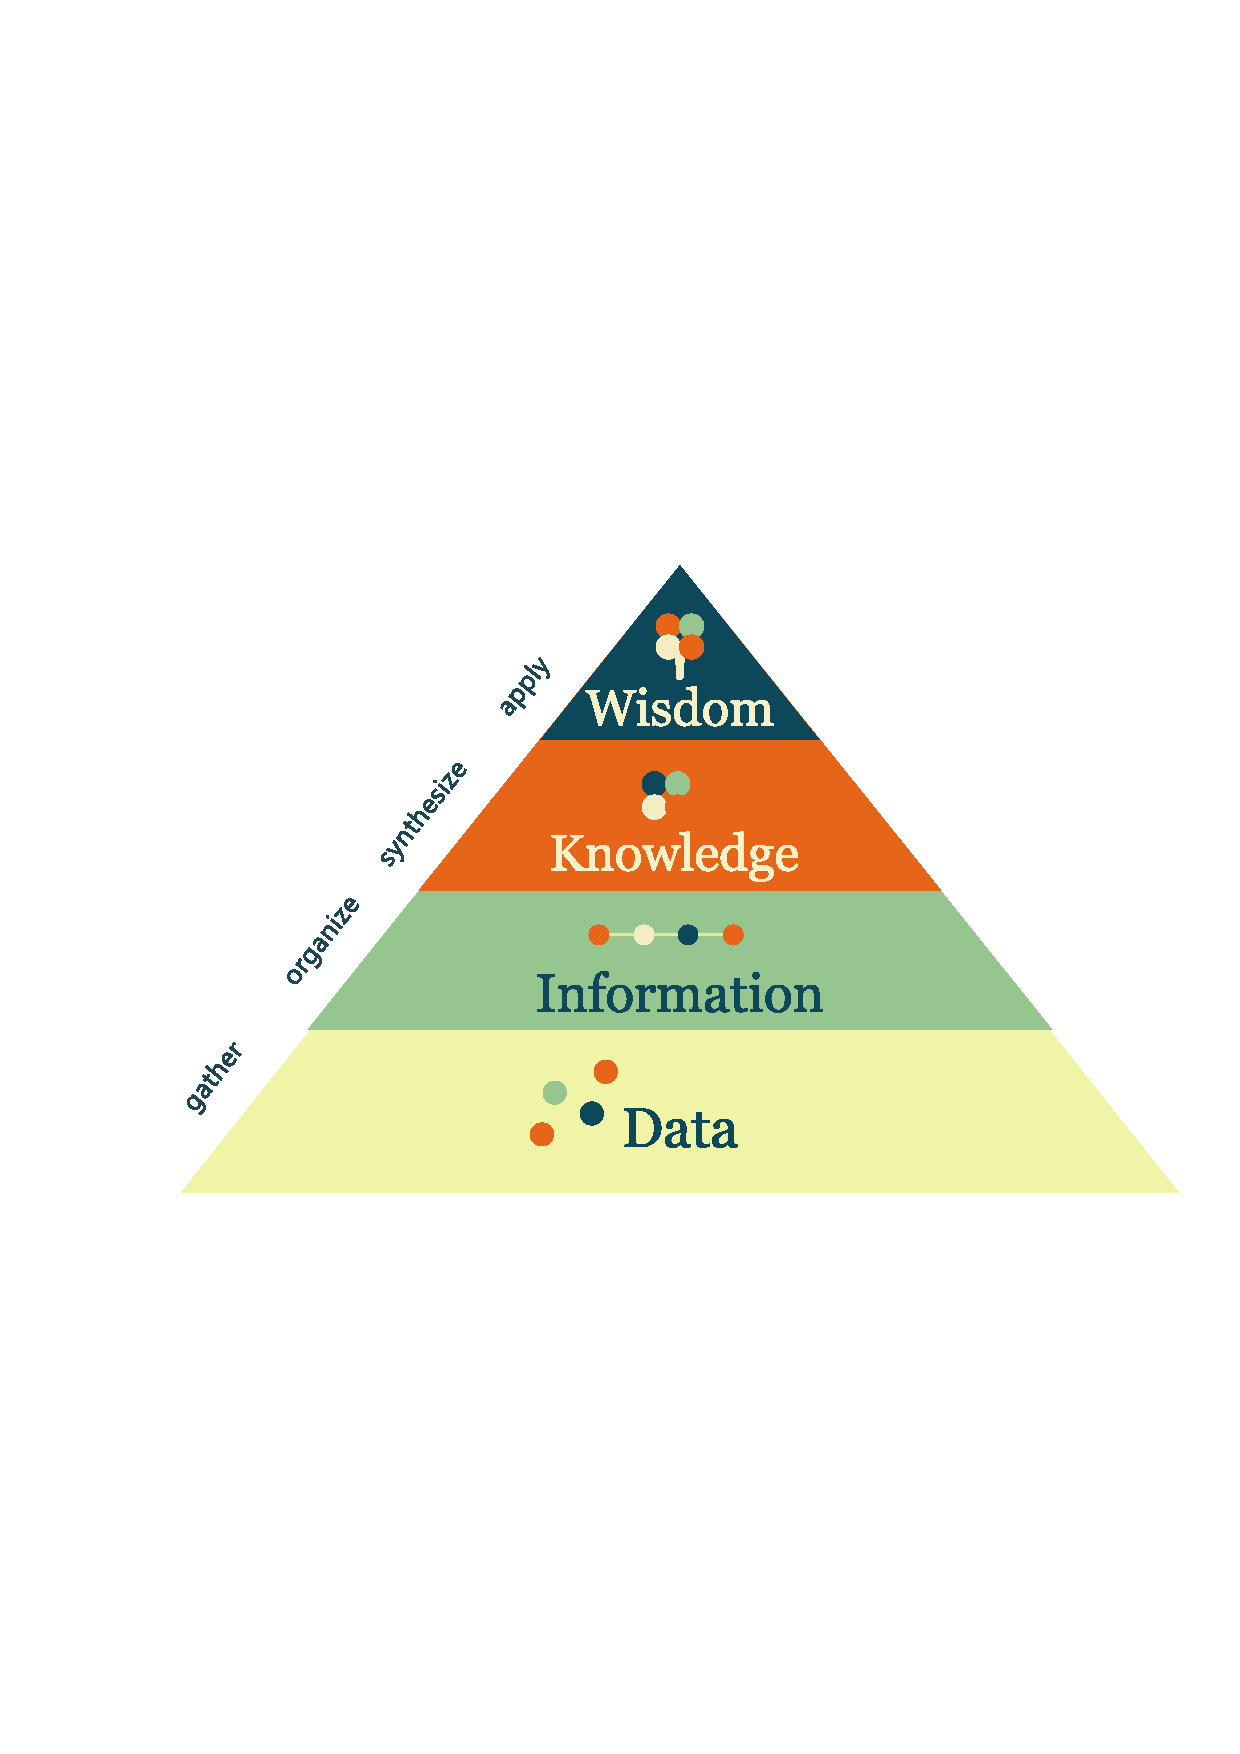
\includegraphics[trim=0 260pt 0 260pt, clip, width=0.75\textwidth]{parts/foundations/images/dikw_pyramid.pdf}
    \caption{Conceptual representation of DIKW pyramid.}
    \label{fig:dikw}
\end{figure}


The relevance of this framework in the context of digitalization lies less in the existence of a strict hierarchy than in the progressive transformation it emphasizes. The increasing value of data derives from the ability to move beyond its mere collection and towards its interpretation and use. Operational databases provide the means to capture observations reliably; analytical infrastructures organize and contextualize them; analytical methods extract patterns and models; and decision-support mechanisms make the resulting knowledge useful for planning and action.

This evolution also changed the requirements imposed on the infrastructures supporting data processing. As long as the principal objective was the reliable recording of operational events, relatively stable schemas and transaction-oriented workloads were sufficient. As data began to be integrated across systems and analyzed historically, systems had to support larger datasets, increasingly complex queries, heterogeneous sources, and transformations between operational and analytical representations.

The growing diversity of digital sources further amplified these requirements. Web applications, distributed software systems, multimedia repositories, machine logs, and eventually sensor infrastructures generated data with substantially greater volume and variety, often without the rigid structures traditionally associated with transactional systems. Data management therefore progressively moved beyond centralized relational databases towards scalable distributed infrastructures capable of storing and processing heterogeneous, semi-structured collections of data.

NoSQL solutions, data lakes and big data platforms emerged in response to these requirements, providing mechanisms for the large-scale storage and distributed processing of heterogeneous data. Later data lakehouse architectures attempted to combine the flexibility of large-scale data storage with stronger transactional, performance, and governance capabilities. Across these developments, a common trend can be observed: as the amount and diversity of data increased, the computational infrastructure had to become increasingly capable of integrating and processing data that could no longer be treated as a small collection of homogeneous, stable records. Consequently, data management in terms of integration and governance became just as important, if not more so, than the ability to efficiently store and retrieve data.

At the same time, the temporal dimension of data became increasingly important. Traditional analytical workloads were predominantly retrospective. They aimed to explain historical behaviour, compare past states, and identify patterns in accumulated records. As digital systems began to generate data continuously, however, a new requirement emerged: information had to be processed while the underlying process was still unfolding.

Streaming architectures consequently introduced a complementary computational model in which data could be ingested, transformed, enriched, and analyzed continuously rather than exclusively through periodic batch execution. The evolution from batch-oriented to continuous processing reduced the temporal distance between the observation of an event and the computational response to it.

This change was particularly relevant for predictive analytics. Once historical data could be combined with statistical and machine-learning methods, information systems were no longer limited to describing what had happened. They could estimate future states, identify emerging conditions, forecast demand, predict failures, and support decisions under uncertainty. The analytical objective consequently shifted from retrospective description towards anticipation.

More recent advances in artificial intelligence extend this trajectory further. Large-scale machine-learning systems can derive increasingly complex representations and predictions from heterogeneous data, while generative AI systems can synthesize information and interact with it through increasingly flexible interfaces. Emerging agentic AI systems further combine these capabilities with reasoning, planning, tool use, and execution. In this setting, data is not merely an input to an isolated analytical process. It becomes part of the context upon which a computational system bases decisions and actions.

The resulting progression can therefore be understood as a gradual reduction in the temporal and conceptual distance between data and action. Early information systems primarily recorded what had happened. Analytical systems transformed accumulated records into information and knowledge. Predictive systems increasingly estimated future states. Agentic AI systems can use such information to support decisions and, in some contexts, participate directly in their execution.

This progression continuously raises the requirements imposed on data management. The larger and more heterogeneous the datasets become, and the closer computation moves towards operational decision making, the more important it becomes that data can be obtained, processed, and interpreted in a timely and reliable manner. The relevant challenge is consequently no longer only how to store more data or process it faster, but how to manage data in ways that preserve its usefulness as it moves across increasingly heterogeneous computational environments.

While continuous data collection and storage techniques have become increasingly mature, the integration and governance of heterogeneous data needed to continuously derive meaningful knowledge and support timely action remain open challenges.

% =========================================================================
\section{From Information Systems to Cyber-Physical Systems}

\label{sec:dss_to_cps}

% =========================================================================

The evolution of data-intensive information systems was accompanied by a progressive expansion of the physical processes that could be digitally observed and computationally managed. Early information systems primarily operated on data generated by organizational activities and transactions. As analytical capabilities matured, these data were increasingly used to support monitoring, planning, and decision making through Business Intelligence, analytical models, and Decision Support Systems (DSS).

The emergence of the Internet of Things (IoT), together with advances in sensing technologies, embedded electronics, communication networks, and distributed computing, progressively extended this computational capability beyond traditional enterprise applications. Physical assets and environments could increasingly be equipped with sensors and connected devices capable of continuously acquiring and transmitting measurements about their state. In the context of Industry~4.0, this pervasive instrumentation became an important enabler of increasingly connected and data-intensive industrial environments.

The availability of continuous physical observations introduced a fundamental change in the relationship between information systems and the processes they represented. Instead of operating primarily on data generated by human or organizational activities, computational infrastructures could increasingly incorporate observations originating directly from the physical processes being monitored. These observations could then be integrated with information systems, analytical models, and decision mechanisms to support increasingly timely responses.

This convergence between information processing and physical processes provided the basis for the development of \textbf{Cyber-Physical Systems} (CPS). CPS are systems in which computational and communication capabilities are tightly integrated with physical processes through sensing and actuation, establishing feedback interactions between their cyber and physical components \cite{lee2008,nist_cps}. In a CPS, computational processes do not merely represent or analyze a physical process, but can continuously observe its state and, through appropriate control mechanisms, influence its evolution. Sensing, computation, communication, and actuation therefore form an integrated loop connecting the physical and cyber domains.

The transition from conventional Information Systems and DSS to CPS can therefore be understood as a change in the role and temporal relevance of data within the computational loop. In traditional information systems, data often describe organizational activities whose relevant state changes on timescales compatible with human decision making and periodic information processing. Pervasive sensing and CPS extend this model to physical processes characterized by substantially different dynamics. Some processes may evolve relatively slowly, allowing observations to be collected, aggregated, and analyzed over relatively long periods. Others may change continuously or rapidly, requiring observations to be processed and decisions to be taken within increasingly short time windows.

This distinction introduces an important temporal dimension to data-intensive systems. As the rate at which physical processes evolve increases, the interval available between observing a system, processing the corresponding information, and taking an appropriate decision becomes progressively smaller. The value of an observation may therefore depend not only on its accuracy or availability, but also on whether it can be acquired, transmitted, interpreted, and acted upon within the relevant temporal window of the physical process. Data management consequently becomes increasingly intertwined with the operational requirements of the systems that generate and consume the data.

At the same time, pervasive digitalization makes physical processes increasingly observable through multiple and independently developed systems. A single physical entity may be described through sensor measurements, information maintained by enterprise systems, engineering models, historical observations, simulation results, and analytical outputs. These sources may differ in structure, semantics, granularity, temporal resolution, and purpose. The challenge is therefore not only to acquire physical observations, but also to maintain meaningful relationships among the different forms of information describing the same physical entity or process.

This requirement motivates a further abstraction of the relationship between physical processes and their digital representations. Rather than treating physical observations only as inputs to individual monitoring or control loops, digital systems can maintain persistent virtual representations associated with physical entities or processes. Such representations can combine information originating from different sources and from different stages of the entity's lifecycle, providing a computational view that can be used for monitoring, analysis, simulation, prediction, and coordination.

This is the conceptual space in which the Digital Twin paradigm has emerged. Digital Twins and CPS should not, however, be understood as successive technologies in a simple evolutionary chain. Rather, they represent complementary perspectives on the digitalization of physical processes. CPS focus on the integration of computation, communication, sensing, and actuation with physical processes, enabling computational systems to observe and influence their operation. Digital Twins focus on maintaining and exploiting digital representations of physical entities or processes, potentially integrating information from multiple systems and over extended periods of their lifecycle. A CPS may therefore incorporate one or more Digital Twins as part of its computational capabilities, while a Digital Twin may operate as a component of a larger cyber-physical environment without itself constituting a complete CPS.

From this perspective, Digital Twins extend the role of digital information beyond the immediate feedback loops of individual cyber-physical systems. A Digital Twin can maintain a persistent and information-rich representation of an entity, combining current observations with historical data, contextual information, models, and analytical results. This representation can subsequently be exploited for purposes that extend beyond real-time control, including simulation, prediction, optimization, lifecycle management, and coordination with other digital representations.

The increasing integration of pervasive sensing, CPS, and Digital Twins therefore changes both the scale and the temporal characteristics of data-intensive systems. Physical processes can be observed continuously, their digital representations can be maintained over time, and computational decisions can increasingly be made within narrow temporal windows. At the same time, these representations may depend on information produced by multiple systems and serving different purposes. The resulting data-management problem is consequently characterized not only by increasing data volumes and velocities, but also by the need to manage heterogeneous information that is continuously produced, consumed, and transformed across interconnected computational and physical processes.

These characteristics motivate the need for data management approaches and software infrastructures capable of supporting Digital Twins as components of larger, interconnected ecosystems. In particular, the ability to integrate information originating from different sources, while respecting the temporal and operational requirements of the physical processes they represent, becomes a fundamental requirement for moving from isolated Digital Twins toward interoperable Digital Twin ecosystems.


% =========================================================================

\section{The Role of Data in a Digital Society}

\label{sec:role_of_data}

% =========================================================================

The developments described above have progressively transformed data from an operational by-product into a strategic resource of the digital economy. Data is now continuously or repeatedly generated by enterprise systems, software applications, connected devices, industrial equipment, and physical infrastructures. Its increasing economic and technological importance is well captured by the expression \emph{``data is the new oil''}\footnote{The phrase is widely attributed to British mathematician and data scientist Clive Humby\cite{humby2006data}.}.

The metaphor is particularly useful because the value of oil does not arise from extraction alone. Crude oil must be transported, refined, and processed before it becomes a useful product. Data follows a similar principle. Raw data has limited value in isolation: it must be collected, stored, transformed, integrated, and interpreted before it can contribute to information, knowledge, and ultimately action. Databases, data warehouses, distributed data platforms, stream-processing infrastructures, and analytical methods can therefore be viewed as the infrastructure through which raw data is progressively transformed into something that can be used.

The scale of this resource has grown rapidly. IoT Analytics estimates 18.5 billion connected IoT devices in 2024 and 21.1 billion by the end of 2025, with approximately 39 billion forecast for 2030\footnote{IoT Analytics, ``State of IoT: Number of Connected IoT Devices,'' \url{https://iot-analytics.com/number-connected-iot-devices/}, updated October 2025.}. Beyond the physical volume of data generated, its economic relevance is also measurable. The European Data Market Study 2024--2026 estimates the EU27 data market at approximately EUR~90 billion in 2024, up from EUR~82 billion in 2023, while the broader data economy, including the direct and indirect economic impacts of data, reached approximately EUR~579 billion in 2024, with a baseline projection reaching approximately EUR~815 billion by 2030 \cite{eudatamarket2024}.

These figures also highlight an important distinction: the value of data does not derive simply from its existence or volume, but from the capability to make it useful. The same principle has accompanied the evolution of information systems throughout the previous decades. Data Warehouses transformed operational records into analytical information; Big Data platforms enabled the management of large heterogeneous datasets; streaming infrastructures enabled continuous processing; and analytical methods transformed accumulated observations into models and knowledge.

The oil metaphor has, however, increasingly been challenged on precisely the dimension of sustainability it seems to evoke. Oil is a finite, extractive resource whose consumption is inherently exhaustible; data, by contrast, is typically assumed to be effectively limitless and immaterial, infinitely copiable at negligible marginal cost, and detached from any physical substrate that could itself be depleted. Taffel critically examines this assumption, arguing that the metaphor implicitly frames digital technologies as clean, renewable, and sustainable, whereas an infrastructural analysis of the material conditions underpinning data reveals a rather different picture: the substantial quantities of energy, minerals, and fossil fuels required to sustain global data infrastructure, together with the environmental costs of its manufacturing and disposal \cite{taffel2021}. From this perspective, the metaphor does not merely simplify; it actively obscures the environmental footprint of the digital economy it purports to describe.

The rapid growth of data centres and, more recently, of artificial intelligence workloads has made this material dimension increasingly difficult to ignore. The International Energy Agency, in a report explicitly examining the relationship between energy demand and artificial intelligence, estimates that data centres consumed approximately 415~TWh of electricity in 2024, around 1.5\% of global electricity consumption, and projects consumption to reach approximately 945~TWh by 2030 in its base case, representing just under 3\% of global electricity demand. The report attributes a substantial share of this growth to the rapid expansion of AI-specific data centres and workloads \cite{iea2025}. In parallel, the 2024 United States Data Center Energy Usage Report estimates approximately 66 billion litres of direct water consumption by US data centres in 2023, compared with 21.2 billion litres in 2014 \cite{shehabi2024}.

These figures make clear that digitalization is not detached from the physical world: digital infrastructures depend on physical resources, energy, communication networks, hardware, and facilities, and their sustainability cannot be taken for granted simply because data itself appears immaterial.

The increasing collection and exploitation of data also raises a further set of concerns, distinct from its material or economic dimensions: questions of privacy, security, ownership, and governance over who may access, combine, and repurpose it. These concerns become more pressing as data increasingly moves across organizational boundaries and independently developed systems, a tendency this thesis returns to when discussing the data governance mechanisms required for Digital Twin Ecosystems in \Cref{chap:data_oriented_perspective}. The greater the scale and pervasiveness of digital observations, the greater the importance of being able to determine and trace how data is collected, processed, shared, retained, and reused.

The increasing importance of data is also accompanied by a change in the type of value expected from it. Historical data remains fundamental for identifying patterns and training models, but modern AI systems increasingly use data to estimate future states, generate recommendations, and support decisions. Emerging agentic AI systems further extend this trajectory by combining information retrieval, reasoning, tool use, and increasingly autonomous execution.

This development does not eliminate the underlying data-management problem. On the contrary, it makes the quality and usability of the data substrate increasingly important. Systems capable of reasoning or acting upon information depend on data to be interpreted correctly, placed in context, and accessed in a timely manner, properties that are often clustered into the data quality concept. As the outputs of computational systems become increasingly connected to operational decisions and physical processes, the consequences of poorly managed or isolated data also become more significant.

The evolution described in this chapter can therefore be read as a progression from data as record to data as resource, and from data as passive representation to data as an active component of computational decision loops. Each of these transitions raised, rather than resolved, the underlying requirement to integrate and govern the resulting data reliably. Digital Twins represent the most recent stage of this progression, maintaining persistent representations of physical entities that draw on multiple sources over their operational lifetime; the specific challenges this raises for independently developed Digital Twins are examined in detail in the next chapter.

This requirement is set to become more pressing, not less. As growing numbers of Digital Twins, and of digital systems more generally, are expected to coexist and collaborate rather than operate in isolation, the data they produce and consume increasingly needs to be shared, reconciled, and jointly interpreted across systems that were never designed together. Meeting this requirement calls for governance mechanisms substantially stronger than those sufficient for a single, self-contained system, covering the quality, provenance, semantics, and access of data as it moves across organizational and technical boundaries. This is not a concern confined to Digital Twins. The same dependence on well-integrated, well-governed data underlies the emerging generation of AI agents: systems that retrieve information, reason over it, and act with increasing autonomy are only as reliable as the data they draw upon. An agent reasoning over incomplete, inconsistent, or poorly governed data does not merely risk a wrong answer; it risks acting on one. Ensuring the integration and governance of data is therefore not a narrow architectural concern, but an increasingly general precondition for extending autonomous computational systems into the physical world without their errors compounding unchecked.

The challenge emerging at this stage is consequently not only how to collect, store, or process increasingly large amounts of data, but how to provide the architectural and data foundations that make its integration and governance possible across independently developed systems.

The following chapters build on this observation. First, the Digital Twin paradigm is examined in greater detail, including its definitions, characteristics, and current implementations, in order to identify the requirements that distinguish Digital Twin environments from traditional information systems. These requirements motivate a subsequent shift towards a data-oriented perspective, in which data models, architectures, and the mechanisms used to structure and manage Digital Twin data become central to achieving interoperability among independently developed Digital Twin systems.


\chapter{Digital Twins}
\label{chap:digital_twins}
The evolution of digital systems described in the previous chapter provides the technological and conceptual context in which the Digital Twin paradigm has emerged. Increasing sensing capabilities, pervasive connectivity, distributed computing, and continuous data processing have made it possible to establish increasingly rich and persistent digital representations of physical entities and processes. Digital Twins build upon these capabilities by connecting physical systems with digital counterparts that can be used for monitoring, analysis, simulation, prediction, optimization, and decision support.

Despite the growing adoption of the term, however, Digital Twin remains a broad and heterogeneous concept. Different communities and application domains have proposed distinct definitions, architectures, and implementation approaches, often reflecting specific technological or operational requirements. This diversity has enabled the development of highly specialized solutions, but has also contributed to a fragmented landscape with limited interoperability between independently developed Digital Twin systems. As a result, the potential benefits of Digital Twins are often constrained by the difficulty of sharing and reusing information across different systems, applications, and domains.

This chapter examines the Digital Twin paradigm from this perspective. It first discusses the historical development of the concept and the heterogeneous interpretations that have emerged around its definition. It then examines reference architectures and the properties commonly associated with Digital Twins, highlighting the increasing complexity of the models, data, and computational capabilities involved. Building on this architectural discussion, it characterizes the data that Digital Twins produce and consume, and the requirements that follow from its unique characteristics. The discussion subsequently turns to the main challenges emerging from the proliferation of Digital Twin solutions. Finally, the chapter considers interoperability and standardization as emerging requirements for moving from isolated Digital Twin implementations towards interconnected Digital Twin ecosystems.

% =========================================================================

\section{History and Definition}
\label{sec:history-and-definition}
% =========================================================================
The Digital Twin concept origins are traced to Michael Grieves' work on Product Lifecycle Management (PLM)~\cite{grieves2014digital} at the beginning of the 2000s, where it was conceived as a virtual representation of a product throughout its lifecycle. The original conceptualisation introduced three fundamental components that characterize a DT, as also shown in \Cref{fig:grieves_dt}:
\begin{itemize}
    \item a \textit{physical space} and its products;
    \item a \textit{virtual space} with virtual representations of the products;
    \item a \textit{connection} between the two spaces, entailing an information flow between the two entities.
\end{itemize}

\begin{figure}[ht]
    \centering
    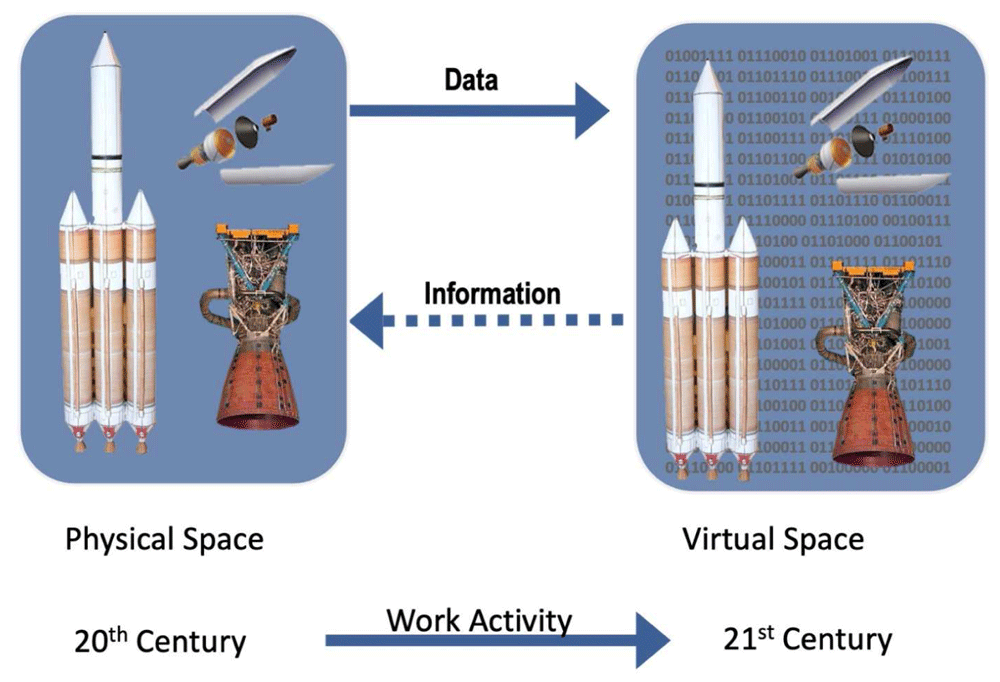
\includegraphics[width=0.65\textwidth]{parts/foundations/images/dt_model_grieves.png}
    \caption{The original DT conceptual model by Grieves, from~\cite{grieves2014digital}} 
    \label{fig:grieves_dt}
\end{figure}

Grieves' early-2000s work is generally regarded as the conceptual origin, while subsequent contributions associated the concept with the term \emph{Digital Twin} and extended it to aerospace and other engineering domains \cite{grieves2002,glaessgen2012,wuni2026}. 

This distinction is important because it places the relationship between the physical and digital spaces at the centre of the concept. The Digital Twin was conceived not merely as a model that could represent a physical object, but as a digital representation connected to it through an ongoing flow of information. In the original formulations, this connection enabled data describing the physical system to be incorporated into the virtual representation, while the information generated within the virtual space could be used to inform decisions concerning the physical system \cite{grieves2014digital,glaessgen2012}.

The subsequent diffusion of the concept was closely related to the development of Industry~4.0, the Internet of Things, industrial connectivity, and data analytics. As physical systems became increasingly instrumented and connected, the continuous acquisition of operational data made it possible to maintain increasingly dynamic digital representations. Digital Twins consequently moved beyond their original product-lifecycle-oriented formulation and were adopted across manufacturing, aerospace, energy, buildings, transportation, healthcare, smart cities, and other domains \cite{qi2021,liu2021,tao2022}.

The growth of the research field reflects this broad diffusion. Tao et al. reported more than 1,000 Digital Twin-related papers per year for three consecutive years beginning in 2019, with 2,934 papers published in 2021 \cite{tao2022}. More recent analyses show an even stronger increase. Wuni et al., analysing scientific and practitioner literature up to 2024, report a substantial growth in Digital Twin publications and identify the last decade as the period in which the vast majority of currently circulating definitions were introduced \cite{wuni2026}. The resulting literature is correspondingly broad, spanning multiple disciplines, application domains, technological approaches, and interpretations of the Digital Twin concept.

This rapid expansion has also created a conceptual problem. As the term has been adopted by communities with different backgrounds and objectives, Digital Twin has increasingly become an umbrella concept encompassing substantially different systems. Different studies may use the same term to describe a simulation model, a three-dimensional representation, a monitoring system, a predictive model, or a fully connected cyber-physical system. Several reviews have therefore identified the lack of a universally accepted definition as one of the persistent challenges of the field \cite{barricelli2019,jones2020,fuller2020,wuni2026}.

\begin{figure}[ht]
    \centering
    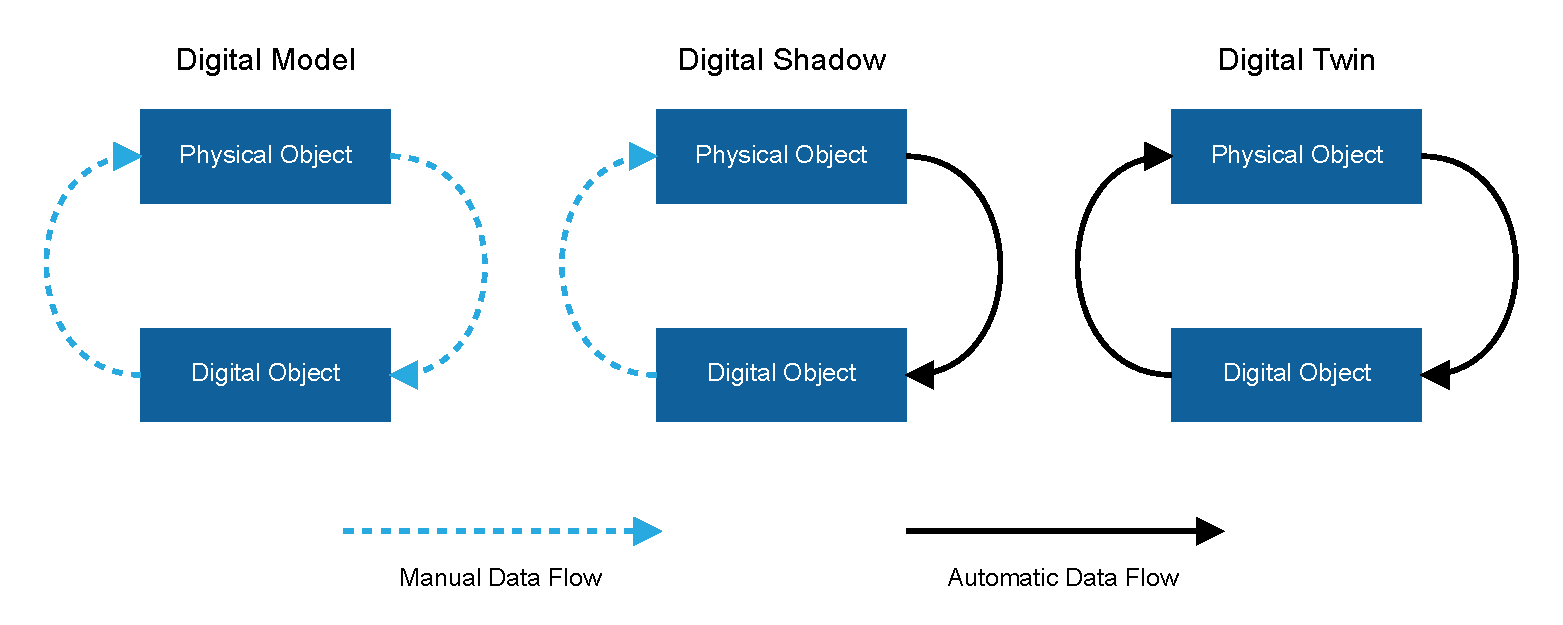
\includegraphics[scale=0.5]{parts/foundations/images/dmdsdt.pdf}
    \caption{Differences between Digital Model, Digital Shadow, and Digital Twin, adapted from Kritzinger et al.~\cite{kritzinger2018}.}
    \label{fig:dtdsdm}
\end{figure}

A particularly useful distinction in this context is the one between a \emph{Digital Model} (DM), a \emph{Digital Shadow} (DS), and a \emph{Digital Twin}, as shown in \Cref{fig:dtdsdm}. Kritzinger et al. introduced this distinction according to the degree and direction of information exchange between the physical and digital entities, a classification subsequently adopted by several reviews and studies \cite{kritzinger2018,fuller2020}. A DM represents a physical entity without an automated connection to it. Changes in the physical system therefore do not automatically propagate to the model, and changes in the model do not automatically affect the physical system.

A DS introduces an automated, but one-directional, connection. Information about changes occurring in the physical system is automatically transferred to the digital representation. The digital representation therefore provides an updated view of the physical system, but does not necessarily influence it automatically. A Digital Twin extends this relationship to bidirectional exchange: changes in the physical system can update the digital representation, while information or decisions generated in the digital space can affect the physical system \cite{kritzinger2018,fuller2020}.

The progression from DM to DT is not primarily determined by the complexity or fidelity of the digital representation, but by the nature and importance of the connection established between the physical and digital entities. A highly detailed three-dimensional simulation that is disconnected from its physical counterpart is therefore not necessarily a Digital Twin, while a less visually sophisticated representation may qualify as one if it is continuously connected to the physical system through an appropriate data flow.

The distinction also highlights the central role played by data in the Digital Twin concept. The transition from DM to DS is enabled by the introduction of an automated data flow, while the transition from DS to DT requires the ability to exchange information in both directions \cite{kritzinger2018,fuller2020}. Communication and data exchange are therefore not merely implementation details; they constitute one of the mechanisms through which the relationship between the physical and digital spaces is established.

Recent systematic analyses provide further evidence of the persistent difficulty of maintaining this conceptual distinction. Wuni et al. analysed 358 definitions from scientific and practitioner sources and found that 66.48\% captured the physical entity, its virtual counterpart, and a persistent bidirectional data and information flow, whereas 33.52\% described entities that, according to their classification, were more appropriately understood as Digital Models \cite{wuni2026}. The analysis also found that terms such as \emph{data}, \emph{information}, \emph{real-time}, \emph{representation}, and \emph{entity} are frequently present in Digital Twin definitions, while terms describing the continuous exchange itself are comparatively less represented \cite{wuni2026}.

This result is particularly relevant to the evolution of the concept. The literature has increasingly recognized that a Digital Twin cannot be reduced to a static representation. Nevertheless, the different formulations used to describe the connection, synchronization, and exchange between physical and virtual entities indicate that the data flow remains interpreted in substantially different ways across the literature. The conceptual core of the Digital Twin is therefore increasingly associated with continuity and synchronization, while the concrete mechanisms through which these properties are modelled and implemented remain strongly dependent on the application domain.

The definition of Digital Twin adopted in this thesis follows this core interpretation.

\begin{quote}
\textit{A Digital Twin is a digital representation of a physical entity or process, continuously connected to its physical counterpart through a bidirectional exchange of information. This enables the digital representation to stay updated with the physical state, while allowing insights generated in the digital space to trigger decisions and actions that directly affect the physical entity.}
\end{quote}

The digital representation may depend on multiple information sources, interact with other digital entities, and expose information that could be relevant to other applications. The more Digital Twins are deployed across interconnected domains, the more important the mechanisms governing their interaction become.

\section{Reference Architectures and Properties}
\label{sec:ref-arch}
% =========================================================================

The increasing adoption of Digital Twins has led to the development of several conceptual models and reference architectures intended to describe their main components and relationships. Although no single architectural representation has emerged as universally adopted, different proposals progressively extend the original conceptualization of the Digital Twin by introducing additional dimensions related to modelling, data, communication, and services \cite{qi2021,tao2022,liu2021}. These models provide useful abstractions for understanding how Digital Twins are structured and how their different components contribute to their operation.

The original formulation introduced by Grieves provided a deliberately simple conceptual representation based on three elements: a physical entity in the physical space, its virtual representation in the virtual space, and a connection enabling information exchange between the two \cite{grieves2014digital}. In this view, the virtual representation provides the digital counterpart of the physical entity, while the connection establishes the relationship through which information can be exchanged. The model therefore captures the fundamental physical--digital relationship underlying the Digital Twin concept.

As Digital Twin applications evolved beyond their original product-lifecycle context, more detailed architectural representations were proposed. One of the most widely referenced models is the five-dimensional Digital Twin model introduced by Tao et al., which extends the original three-part conceptualization by explicitly identifying five dimensions: \textit{physical entity}, \textit{virtual model}, \textit{connection}, \textit{data}, and \textit{service} \cite{tao2019,qi2021}. The model is illustrated in \Cref{fig:tao_dt}.

\begin{figure}[ht]
    \centering
    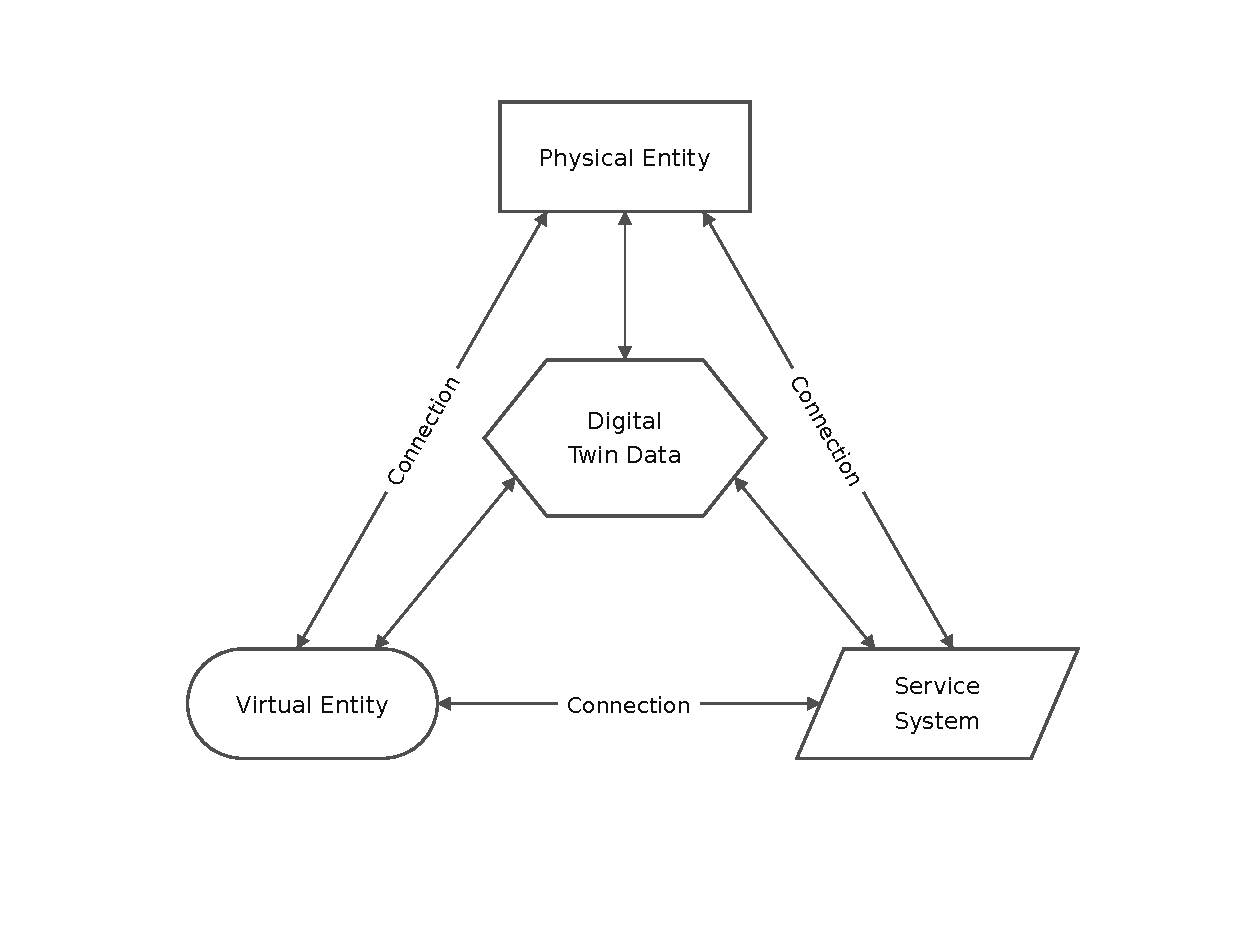
\includegraphics[scale=0.5]{parts/foundations/images/5dim_dt.pdf}
    \caption{Five-dimensional Digital Twin model, adapted from Tao et al.~\cite{tao2019,qi2021}.}
    \label{fig:tao_dt}
\end{figure}

The five-dimensional model provides a more comprehensive architectural view of a Digital Twin. The \textit{physical entity} represents the real-world object, system, or process being twinned, while the \textit{virtual model} provides its digital representation. The \textit{connection} establishes the communication between the physical and virtual spaces, enabling the exchange of information. The \textit{data} dimension captures the information generated, collected, and processed throughout the operation of the Twin, while \textit{services} represent the functionalities offered through the Digital Twin.

Within this model, the virtual representation is not necessarily limited to a single type of model. Tao et al. distinguish geometric, physical, behavioural, and rule models as complementary dimensions that can be combined to represent different aspects of the physical entity \cite{tao2022}. Geometric models describe the shape and structural characteristics of an entity; physical models capture relevant physical properties and constraints; behavioural models describe its dynamic evolution; and rule models incorporate rules, historical information, and domain knowledge. Depending on the application, these models can support simulation, prediction, optimization, diagnosis, and other computational functions.

The explicit introduction of data as a separate dimension, and specifically placed at the core of the architecture,  is particularly relevant to the evolution of Digital Twins. In the original three-component formulation, data was implicitly associated with the connection between the physical and virtual spaces. In the five-dimensional model, it is instead represented as an independent and pivotal architectural element connecting the physical entity, virtual model, connection, and services \cite{qi2021,tao2022}.

Data is therefore involved throughout the operation of a Digital Twin. Measurements and observations produced by the physical entity can be collected and used to update its virtual representation. Historical information can complement current observations, while data-driven and model-based techniques can transform these inputs into higher-level information and knowledge. The resulting outputs can support services such as monitoring, simulation, prediction, optimization, and decision making \cite{qi2021,tao2022}. Finally, outputs produced within the virtual representation can in turn be used to determine actions affecting the physical entity.

As shown in numerous research articles, the diversity of application domains has consequently resulted in a wide range of Digital Twin architectures and implementations. Tao et al. reviewed 284 publications on Digital Twin models and found that almost half concerned manufacturing applications. Energy represented 35 publications and aerospace 20, while further applications were identified in areas such as engineering construction, cities, healthcare, transportation, and environmental systems \cite{tao2022}. This distribution illustrates the progressive diffusion of the concept from its initial engineering and manufacturing context towards a much broader set of application domains.

Architectural variation also emerges from the scale of the physical systems being represented. Tao et al. distinguish between unit-level, system-level, and System-of-Systems (SoS)-level Digital Twin models \cite{tao2022}. At the unit level, a Twin may represent an individual component or piece of equipment. At the system level, it may represent a production line, aircraft subsystem, building, or other integrated system composed of multiple components. At the SoS level, the Digital Twin represents a collection of interacting systems whose behaviour depends on the relationships between their constituent parts.

This hierarchical perspective is particularly relevant to the architecture of complex Digital Twin Ecosystems (DTE).
%
The idea of bringing multiple Digital Twins together traces back to Grieves, who envisioned aggregating homogeneous DT instances to observe population-level behaviors and trends across identical products~\cite{Grtz2026}. In contrast, the modern framing of a DTE as an ecosystem of heterogeneous Digital Twins is largely shaped by the UK's National Digital Twin programme.
%
Under this paradigm, the National Digital Twin is defined as “an ecosystem of digital twins and the protocols by which they can be integrated securely and resiliently”~\cite{dtarch}. 
%
A Digital Twin at one level may therefore coexist with other Twins representing related entities at different levels of abstraction. In a manufacturing environment, for example, individual machines may be represented by dedicated Digital Twins, while a production line may be represented at a higher level by a Twin that considers the interactions among those machines. Similar hierarchical relationships can be found in other domains, such as aerospace, healthcare, and urban systems \cite{tao2022}.

Recent reference architectures have increasingly conceptualized the Digital Twin not as a tailored, self-contained entity, but as a modular platform component governed by service-oriented principles. Aligning with this perspective, Aheleroff et al. \cite{AHELEROFF2021101225} proposed a \emph{Digital Twin as a Service} (DTaaS) reference model for Industry 4.0. Their work highlights the necessity of abstracting DT functionalities into scalable, cloud-based services to support complex system integration across a large number of assets. Crucially, this DTaaS approach acts as an architectural blueprint: rather than dictating a monolithic structure, it identifies the mandatory infrastructural modules required to operate a DT. By standardizing these core components into composable building blocks, the architecture empowers developers to flexibly assemble, instantiate, and scale customized Digital Twins. Consequently, the development focus shifts from engineering isolated systems from scratch to leveraging a shared, service-oriented infrastructure that inherently fosters standardization and interoperability.

Across these different approaches, the specific technologies and internal structures may vary considerably, but several architectural elements recur: a physical entity, a digital representation, mechanisms for exchanging information between the two, data supporting the representation and its operation, and services built on top of the available models and information. The balance among these elements depends strongly on the domain, the characteristics of the physical system, and the intended functionality of the Digital Twin.

The literature therefore presents the Digital Twin not as a single architectural pattern, but as a family of related architectural abstractions. The original three-component model provides a conceptual foundation centered on the physical--digital relationship, while subsequent models introduce additional dimensions to capture the data, models, and services required by increasingly sophisticated implementations. In particular, the explicit introduction of data as an architectural dimension represents an important step in the evolution of the concept, reflecting the increasing role of information in maintaining, operating, and exploiting Digital Twins. Having recurred, in every reference architecture discussed above, as the element connecting the physical entity, its virtual representation, and the services built on top of it, data deserves to be examined in its own terms as the basis for the data-oriented perspective developed in the remainder of this thesis.

\section{Challenges and Opportunities}

\label{sec:challenges}

The increasing adoption of Digital Twins across different application domains introduces significant opportunities for monitoring, analysis, simulation, optimization, and decision support. At the same time, the current state of development of Digital Twins presents several challenges related to their increasing \textit{complexity} and wide \textit{heterogeneity}. In terms of heterogeneity, DTs may differ with respect to the physical systems they represent, the goals they pursue, the data they rely on, and most notably, the technologies and architectures used for their implementation.
%
Some of these differences are the result of the limited degree of \textit{standardization} achieved so far, despite the research community having strongly advocated for greater standardization efforts over the last decade \cite{wang2022standards,wuni2026}.
%
While the number of publications related to DTs has increased extremely rapidly, the literature shows that some studies still fail to provide a clear definition of the DT concept and consequently, at least partially, fail to reflect its essential characteristics in their implementations. Others provide definitions that are not consistent with one another \cite{wuni2026,tao2022}.
%
The lack of standardization also hinders the development of frameworks, reference architectures, and platforms capable of supporting the development of DTs in a consistent and modular way.
%
Furthermore, if standardization is already a challenge within individual DTs, its absence becomes even more relevant when considering more complex scenarios such as DTEs, in which multiple DTs are expected to coexist and meaningfully interact.

The meaningful interaction required within DTEs introduces a further challenge related to \textit{interoperability}. Independently developed DTs need to be able to communicate and exchange information in a way that is meaningful for all the systems involved. This requires not only a technical connection between the systems, but also a shared understanding of the exchanged information, including its semantics and context. Interoperability is therefore a multi-level challenge encompassing technical, syntactic, and semantic aspects, and requiring mechanisms to manage differences between independently developed systems.

Heterogeneity and the resulting lack of coordination between independently developed Digital Twins are, in this sense, the root of the problem. Addressing them requires progress along two related fronts. \textbf{Standardization} is the primary lever available for this purpose: the definition of common principles, structures, and mechanisms that can provide shared foundations for developing and managing Digital Twins, thereby reducing unnecessary heterogeneity. \textbf{Interoperability} is the capability such foundations are meant to enable: the ability of different, independently developed Digital Twins to communicate, exchange information, and cooperate effectively. Standardization and interoperability are therefore closely related (the former is typically a precondition for the latter) but they address different aspects of the problem and, as discussed below, are not always achieved together.
%
These two dimensions will be discussed from two different perspectives: single Digital Twins and Digital Twin Ecosystems. The former primarily concerns the development of individual Digital Twins, while the latter concerns the interaction between multiple independently developed Digital Twins.

\subsection{Standardization}

At the level of an individual Digital Twin, standardization can provide a common foundation for its construction and management. Rather than defining every Digital Twin as a completely independent solution, standardized building blocks, architectural principles, and mechanisms can guide developers in assembling the components required by a particular application. Such standardization does not require all Digital Twins to have the same structure or capabilities. Instead, it can provide a common set of elements from which different Digital Twins can be constructed and tailored to their specific requirements.

At the level of a Digital Twin Ecosystem (DTE), the scope of standardization becomes broader. A DTE involves multiple Digital Twins that may have been developed independently and may rely on different technological solutions. Standardization can therefore concern the common foundations of the ecosystem itself, including the infrastructure, architectural principles, interfaces, and data representations that support the deployment and interaction of multiple Digital Twins. In this sense, standardization can reduce unnecessary differences between implementations and provide a common basis on which heterogeneous Digital Twins can coexist.

Wang et al. review the landscape of Digital Twin standardization efforts, consolidating contributions from organizations including the International Organization for Standardization (ISO), the International Electrotechnical Commission (IEC), the International Telecommunication Union (ITU), and the Institute of Electrical and Electronics Engineers (IEEE) \cite{wang2022standards}. Their review is framed around the five-dimensional Digital Twin model introduced by Tao et al., comprising the physical entity, virtual model, connection, data, and services \cite{tao2019,qi2021}. For the purposes of this thesis, two of these dimensions are particularly relevant: the \textit{connection}, which provides the infrastructural basis for communication and interaction, and \textit{data}, which constitutes the information exchanged and processed by the different components of the Digital Twin.

From an infrastructural perspective, standardization addresses the mechanisms through which Digital Twins and their components can connect and communicate. Common interfaces, communication protocols, service descriptions, and architectural principles can reduce implementation-specific dependencies and facilitate the integration of independently developed components. Wang et al. identify the lack of common references for Digital Twin architectures and communication mechanisms as an important obstacle to the interconnection of Digital Twin components and services across different systems and domains \cite{wang2022standards}. Standardization at this level therefore provides the technical foundations required for Digital Twin systems to communicate.

A second and complementary dimension concerns the data exchanged through these infrastructures. Digital Twins continuously produce, consume, and transform information originating from physical entities, models, sensors, information systems, and other computational services. Wang et al. identify several standardization requirements related to Digital Twin data, including the processing of heterogeneous data, the management of multi-source and multi-modal data, and mechanisms concerning data syntax, semantic mapping, and data exchange \cite{wang2022standards}. These requirements indicate that standardization cannot be limited to the mechanisms used to transport data; the representation and interpretation of the exchanged information are equally, if not more so, relevant.

These two dimensions of standardization, of the infrastructure used to connect Digital Twins, and of the data they exchange, do not exhibit the same degree of maturity. Communication and interface standards provide increasingly established mechanisms through which heterogeneous systems can connect, while data-oriented standards and semantic approaches are comparatively less developed \cite{wang2022standards}. This gap becomes especially relevant within a Digital Twin Ecosystem: while an individual Digital Twin can often rely on tightly coupled, internally consistent interfaces and data representations, a Digital Twin Ecosystem brings together systems designed around different assumptions, so that establishing a communication channel between them is only a first step. Standardizing that channel does not, by itself, guarantee that the information exchanged through it will be correctly interpreted by the receiving system.

From this perspective, standardization should not be understood as an attempt to impose a single implementation on all Digital Twins. Domain-specific models, technologies, and services may remain necessary to address the characteristics of individual physical systems. The objective is instead to identify and standardize the common elements at the boundaries between systems, allowing Digital Twins to retain their internal specialization while remaining capable of participating in a broader ecosystem. Achieving such common foundations can reduce the effort required to develop new Digital Twins, facilitate their integration, and enable the reuse of data and services across applications. It can also support the development of reusable frameworks and platforms capable of deploying and managing Digital Twins according to shared architectural principles.     However, providing common foundations does not, by itself, guarantee that independently developed Digital Twins can effectively work together. This motivates the following discussion, which considers interoperability as a distinct challenge in its own right.

\subsection{Interoperability}

Interoperability becomes particularly relevant at the level of the Digital Twin Ecosystem. When multiple Digital Twins are independently developed, they may rely on different architectures, interfaces, data representations, and terminology. The challenge is therefore to enable these systems to communicate seamlessly and to exchange information that can be correctly understood and used by the receiving system.

At the level of an individual Digital Twin, there is no interoperability problem in the sense of interaction between independently developed Digital Twins, since the system is considered in isolation. Internal components still need to interact with one another, but this is primarily a matter of designing and integrating the Digital Twin itself. Interoperability becomes a distinct concern when multiple Digital Twins are brought together within a DTE.

This distinction is important because interoperability does not simply mean connecting systems despite their differences. Rather, it concerns finding ways to integrate those differences so that independently developed systems can communicate and make meaningful use of the information exchanged between them. A system should not merely receive a message from another system; it should be able to understand what that information represents and use it within its own context.

This requirement becomes particularly important when Digital Twins exchange information that contributes to monitoring, analysis, or decision-making. Two systems may use different representations for the same physical phenomenon, and a successful interaction requires more than a technical connection between them. The receiving system must be able to interpret the exchanged information according to its intended meaning and context.

Recent literature has begun to characterize this problem more precisely, distinguishing between several levels at which interoperability between Digital Twins can be assessed and pursued. Acharya et al.~\cite{acharya2024interoperability}, surveying interoperability within Digital Twin deployments in cyber-physical systems, delineate distinct interoperability levels and examine the challenges associated with each. Their analysis proposes a framework of six such levels, namely \textit{technical}, \textit{syntactic}, \textit{semantic}, \textit{pragmatic}, \textit{dynamic}, and \textit{organizational}, which range from the basic ability of Digital Twins to exchange messages over a common communication infrastructure, through agreement on a common structure and encoding for the exchanged data, up to the higher-level ability to agree on the meaning of the exchanged concepts and on the business or operational context in which they are used. For the purposes of this thesis, the technical, syntactic, and semantic levels are the most directly relevant, since they map most closely onto the software/data distinction followed here.
%
David et al. similarly review the challenges affecting interoperability among Digital Twins, together with the factors that have been found to contribute to successful interoperable deployments, and outline directions for future research on the topic \cite{david2024interoperability}. Both contributions confirm that achieving interoperability across independently developed Digital Twins requires more than establishing a technical connection between them.

A simple example makes the semantic level concrete: two Digital Twins monitoring similar physical processes may represent the same measured quantity, such as temperature, under different property names, units, or data structures. A compatible communication channel is sufficient to transmit the corresponding value from one system to the other, but it does not by itself guarantee that the receiving system correctly identifies what that value represents; establishing this correspondence is a matter of semantic, rather than merely technical or syntactic, interoperability.

Standardization and interoperability therefore address complementary aspects of the same underlying problem: the former provides shared architectural and data-related foundations for constructing Digital Twins and Digital Twin Ecosystems, while the latter concerns the ability of independently developed Digital Twins to exchange and meaningfully reuse each other's information once such foundations are in place. The following chapter examines this problem from the perspective of the data involved, characterizing the data that Digital Twins produce and consume and the mechanisms required to manage it consistently across independently developed systems.

\chapter{A Data Oriented Perspective}
\label{chap:data_oriented_perspective}
This chapter adopts a data-oriented perspective on the standardization and interoperability challenges discussed in the previous chapter. It first argues for treating the data and software dimensions of a Digital Twin as separable, complementary design concerns, and examines how the two challenges just discussed relate to this separation. It then characterizes the data that Digital Twins produce and consume, discussing the requirements that follow from the diversity of the domains in which Digital Twins are deployed. Finally, building on this characterization, it examines the architectural and semantic foundations required to support such data across individual Digital Twins and Digital Twin Ecosystems.

\section{Divide et Impera}

Digital Twins, and the platforms that support them, can be described along two complementary dimensions: a \textit{software} dimension, concerned with the applications, services, and infrastructural components through which Digital Twins are deployed, executed, and made accessible; and a \textit{data} dimension, concerned with the information that Digital Twins collect, process, store, and exchange. These two dimensions are not independent, but modular and complementary. Every software component of a Digital Twin, from the simplest monitoring dashboard to the most sophisticated simulation service, ultimately operates on data: it acquires it, transforms it, and produces new data to be stored and eventually consumed elsewhere. In this sense, the software dimension of a Digital Twin can be regarded as a layer of applications built on top of the data dimension, rather than as an independent architectural concern.

This observation motivates a deliberate decomposition of the problem. Rather than addressing the software and data dimensions jointly, and thereby risking the reproduction of the same fragmentation already observed in existing Digital Twin implementations, this thesis separates the two concerns and concentrates on the data dimension. This choice is not intended to diminish the relevance of software architectures, which remain necessary to deploy, orchestrate, and expose Digital Twin functionalities. It reflects, instead, the observation that many of the interoperability difficulties discussed in the previous chapter originate not from the diversity of software implementations per se, but from the heterogeneity of the underlying data: its models, schemas, semantics, and governance \cite{acharya2024interoperability,david2024interoperability}. Two Digital Twins built on entirely different software stacks can still interoperate if they share a common understanding of the data they exchange, whereas two Digital Twins built on the same software stack may fail to interoperate if their underlying data representations are incompatible.

This separation can be made more concrete by revisiting the standardization and interoperability challenges discussed in \Cref{sec:challenges}. \Cref{tab:standardization_interoperability} decomposes each of these challenges, at both the individual Digital Twin and the Digital Twin Ecosystem level, into a software-related and a data-related component. In each cell, the software-related component concerns the mechanisms through which components are built or connected, such as architectural building blocks, communication protocols, and interfaces, which are increasingly addressed by existing reference architectures and standardization efforts \cite{wang2022standards}. The data-related component concerns instead the models, representations, and shared meaning of the information involved, and is comparatively less mature, particularly at the Digital Twin Ecosystem level: standardizing a communication protocol does not by itself guarantee that the resulting data can be modelled consistently or interpreted uniformly across independently developed Digital Twins. This asymmetry motivates the choice, introduced above, to concentrate the remainder of this thesis on the data dimension.

\begin{table}[htbp]
\centering
\caption{Standardization and interoperability challenges at the Digital Twin (DT) and Digital Twin Ecosystem (DTE) levels, decomposed into their software and data components.}
\label{tab:standardization_interoperability}
\renewcommand{\arraystretch}{1.5} % Leggermente aumentato per far respirare il testo
\begin{tabular}{p{3.2cm} p{5.5cm} p{5.5cm}}
\toprule
\textbf{Challenge} & \textbf{DT} & \textbf{DTE} \\
\midrule
\textbf{Standardization} 
& 
\textit{Software:} architectural principles, building blocks. \newline
\textit{Data:} data models, transformation methodologies and metadata management.
& 
\textit{Software:} shared infrastructure, protocols, interfaces. \newline
\textit{Data:} common data models and schemas, DTP.
\\
\addlinespace
\textbf{Interoperability} 
& 
\textit{n/a}
& 
\textit{Software:} communication protocols, interface standards. \newline
\textit{Data:} common semantics, shared governance and metadata management.
\\
\bottomrule
\end{tabular}
\end{table}

Furthermore, the modularity between the data and software dimensions allows research to be conducted individually on each of them, without requiring the other to be addressed simultaneously. This thesis concentrates on the data dimension, while acknowledging that the software dimension remains a necessary complement to it.

Before this data dimension can be supported by an appropriate platform, however, it must first be understood on its own terms: what kinds of data Digital Twins actually produce and consume, and what requirements follow from their specific characteristics. The next section explores this question.

\section{Digital Twin Data}
\label{sec:dt_data}

Data occupies a distinctive position among the elements that make up a Digital Twin~\cite{tao2022}. Unlike the physical entity or the virtual model, which are specific to a given application, data is the element through which every other component of a Digital Twin operates and interacts: it is what the physical entity produces, what the virtual model consumes and updates, what services are built upon, and what is exchanged whenever two Digital Twins communicate. Liu et al. note that data plays a central role in constructing virtual models, establishing cyber-physical connections, and supporting the operation of a Digital Twin \cite{liu2022dtd}. At the same time, the properties that distinguish a Digital Twin from a conventional simulation or a Digital Shadow, discussed in \Cref{sec:history-and-definition}, impose requirements on this data that are not typically found in other data-intensive applications. Characterizing this data, before deciding how to manage it, amounts to a form of domain understanding: just as data-intensive projects typically begin by examining the domain and the data available before committing to a specific modelling or engineering approach, addressing Digital Twin data management must begin by examining what this data actually looks like.

\subsection{Requirements on Digital Twin Data}

From the perspective of its data and at a conceptual level, a Digital Twin can be described, in most cases, in quite simple terms: a physical entity/environment monitored through sensors, whose observations are processed by models or, increasingly, by machine learning/AI components, and whose outputs are in turn used to act on the physical entity. This description makes explicit why the software and data dimensions introduced above are complementary rather than independent: the models and services built on top of a Digital Twin are only as effective as the data made available to them, and their outputs are only as meaningful as they can be related back to the physical entity being monitored.

What varies substantially across applications is the specific type of data involved in this loop, and the requirements it imposes. In manufacturing, discussed in \Cref{sec:ref-arch} with reference to the five-dimensional Digital Twin model, this typically includes sensor measurements from machines and production lines alongside geometric models of the manufactured parts \cite{tao2022}. In the automotive domain, Deng et al. review Digital Twin applications spanning vehicle design, production, transportation, and battery management, in which data ranges from structured diagnostic and telemetry signals, such as those used for battery state monitoring, to the higher-frequency data required for real-time production monitoring and control \cite{deng2023automotive}. In precision agriculture, Zhang et al. describe Digital Twins that combine environmental and soil sensor data with remote sensing imagery to support decisions over considerably longer, biologically determined time scales, and report that fragmented data sources and inconsistent data formats remain a significant obstacle to their integration \cite{zhang2025agriculture}.

These examples illustrate that the requirements imposed by Digital Twin data are extremely shaped by the domain of application. Liu et al. observe more generally that Digital Twin data also exhibits the volume, variety, and velocity commonly associated with big data \cite{liu2022dtd}: volume, because Digital Twins are typically built around densely instrumented entities that generate data continuously; variety, because of the heterogeneity of sources, domains, and data types illustrated above; and velocity, because different parts of the same Digital Twin may require different processing latencies, from near-real-time control loops to periodically updated maintenance records. A further concern, raised in the agricultural example above and identified by Ouedraogo et al. as one of the central challenges in Digital Twin data management, is data quality: sensor-originated data is subject to noise, faults, and calibration issues, which existing data management architectures and techniques need to account for explicitly \cite{ouedraogo2025dtdm}.

These characteristics motivate the more specific requirements identified in the literature. Liu et al. translate them into concrete requirements on Digital Twin data gathering, mining, fusion, interaction, iterative optimization, and on-demand usage \cite{liu2022dtd}.

\subsection{Categorizing Digital Twin Data}
\label{sec:dt_data_categories}

Beyond its heterogeneity, Digital Twin data can be organized along two complementary dimensions found in the literature, each of which has direct consequences on how such data should be modelled and managed.

A first, widely adopted distinction, introduced by the ISO 23247-3 standard for the digital representation of manufacturing elements, separates \emph{static information}, which does not change over the course of the entity's operation, such as its identification or nominal characteristics, from \emph{dynamic information}, which changes as the physical entity operates, such as its status, location, or the current shape of a piece of material undergoing a manufacturing process \cite{liu2022dtd}. Establishing this distinction for a given Digital Twin is itself an exercise in domain understanding, since it clarifies, ahead of any implementation choice, which parts of the data behave as reference or master data, typically low in volume and velocity and well suited to conventional, schema-based representations, and which parts behave as high-velocity, continuously generated observations, more naturally modelled as time-series or event data and requiring correspondingly different storage and processing mechanisms. In this sense, the static/dynamic distinction anticipates some of the data modelling requirements addressed in the remainder of this thesis, and in particular the separation between graph and time-series data adopted in \Cref{chap:stgraph}.

A second, complementary categorization organizes Digital Twin data according to where, within a Digital Twin, it originates. Liu et al. distinguish six such categories: \emph{physical entity-related data}, such as sensor measurements describing equipment, materials, or workers; \emph{virtual model-related data}, such as the parameters, processes, and outcomes of simulation models; \emph{service-related data}, produced by the algorithms and analytics built on top of the Digital Twin; \emph{domain knowledge}, encoding rules, standards, and expert experience; \emph{connection data}, which relates corresponding pieces of physical entity-related and virtual model-related data, such as a real, sensor-measured temperature and the corresponding value simulated by a virtual model; and \emph{fusion data}, obtained by combining the previous categories into a more complete representation of the physical entity \cite{liu2022dtd}.

From a data engineering perspective, these six categories can be read as occupying different layers of a data architecture, echoing the classic distinction between data, information, and knowledge \cite{ackoff1989}. Physical entity-related and virtual model-related data sit at the \emph{raw data} layer: they are the raw observations and simulation outputs produced, respectively, by the physical and the virtual side of the Digital Twin. Connection and fusion data sit one layer above, at the \emph{reconciled} layer: they combine and integrate these raw observations into a coherent, contextualized representation of the physical entity, with fusion data in particular constituting the integration layer at which a Digital Twin's overall view of its physical counterpart is assembled. Service-related data and domain knowledge sit at the \emph{knowledge} layer: the former encodes the outputs of analytics and algorithms applied to the underlying information, while the latter encodes rules and expertise external to any single observation; together, they are what ultimately supports the decisions and actions a Digital Twin takes on its physical entity.

This layered reading has a direct consequence for the data models discussed later in this chapter. A data model intended to support meaningful interoperability across Digital Twins cannot be designed solely around raw, entity- or model-related observations, since these are, by construction, specific to each Digital Twin's own sources. It must instead operate at the information layer, where connection and fusion data already provide a reconciled representation of the physical entity, largely independent of how that entity happens to be sensed or simulated.

Ouedraogo et al. observe that the specific data management considerations arising from this heterogeneity differ across application domains, such as manufacturing, smart cities, and healthcare \cite{ouedraogo2025dtdm}, reinforcing the earlier observation that the variety of Digital Twin data is compounded, rather than absorbed, by the variety of domains in which Digital Twins are deployed.

Taken together, these categorizations show that even a single Digital Twin already involves several qualitatively different types of data, produced and consumed by different components, at different rates, and for different purposes, and that its origin, its layer within the data-information-knowledge architecture just outlined, and its position along the static/dynamic spectrum all carry direct implications for how it should be modelled. This internal heterogeneity is compounded, at the level of a Digital Twin Ecosystem, by the differences in data models, schemas, and semantics adopted by independently developed Digital Twins, discussed in \Cref{sec:challenges}. Characterizing Digital Twin data along the dimensions introduced in this section therefore provides the domain understanding necessary not only for designing the data management capabilities of an individual Digital Twin, but also for identifying the requirements that must be satisfied to support Digital Twin Ecosystems more broadly.

\section{Digital Twin Platform}
\label{sec:dtp}

The definition of Digital Twin Platform adopted in this thesis is the following.

\begin{quote}
\textit{A Digital Twin Platform (DTP) is a software environment that hosts and supports Digital Twins throughout their lifecycle, from deployment to decommissioning, by providing the data management mechanisms they require in terms of infrastructure, data models, and governance.}
\end{quote}

What distinguishes the perspective adopted in this thesis is not whether a DTP is a software environment, but what it is organized around: rather than being structured around the specific software modules and services that make up the Digital Twins it hosts, it is structured around the data those Digital Twins produce and consume. 

This distinction has a direct practical consequence. A Digital Twin Platform designed in this way is largely independent of the internal architecture of the Digital Twins deployed on top of it: the platform does not need to know how a given Digital Twin is implemented internally, only that the data it produces and consumes conforms to the platform's data models and semantic representation standards. A Digital Twin built according to these data models and semantic standards will run on the platform and be able to interoperate with other Digital Twins built the same way, regardless of the specific software stack each of them uses internally. Standardizing on data models and data representations, rather than on software architectures, is therefore the foundation on which this thesis proposes to standardize Digital Twins; the software components of a Digital Twin, whatever their specific architecture, are consequently treated as applications that operate on top of a shared data foundation, rather than as the primary object of standardization.

A Digital Twin Platform, in this sense, does not require every Digital Twin to follow an identical architecture. Its role is instead to provide common capabilities and abstractions that reduce fragmentation and facilitate the construction and management of heterogeneous Digital Twin environments, representing a technological foundation upon which different Digital Twins can be built and, ultimately, connected to one another.

This characterization does not contradict the reference architectures discussed previously, such as the five-dimensional Digital Twin model, in which data already occupies a central, connective role among the physical entity, virtual model, connection, and service dimensions \cite{qi2021,tao2022}. Rather, it makes this centrality explicit at the level of the platform, and uses it as an organizing principle for the remainder of the thesis. Similarly, this perspective is consistent with service-oriented reference models such as Digital Twin as a Service, in which Digital Twin functionality is exposed through composable, standardized building blocks \cite{AHELEROFF2021101225}; in the perspective adopted here, however, the building blocks that are standardized in the first instance are those governing the underlying data, with services constructed on top of them.

Treating data as a first-class citizen in this sense means that the requirements and characteristics of Digital Twin data, discussed in \Cref{sec:dt_data}, are taken as the primary drivers of platform design, rather than as a consequence of decisions made at the software or application level. In many existing systems, data models, storage solutions, and integration mechanisms are chosen to satisfy the immediate needs of a specific application, and are only subsequently, if at all, reconciled with the requirements of other applications or Digital Twins operating on related data. This application-centric approach tends to reproduce, at the level of the platform, the same fragmentation already observed among independently developed Digital Twins. The perspective adopted in this thesis inverts this relationship: the characteristics of Digital Twin data are analysed independently of any specific application, and are used to define the data management capabilities that a Digital Twin Platform should provide, with software applications, including the Digital Twins themselves, developed on top of these capabilities rather than dictating them.

The remainder of this chapter details two complementary aspects of this data-oriented view of the Digital Twin Platform: the architectural and infrastructural foundations required to support Digital Twin data, referred to as data platforms; and the data models and governance mechanisms required to give this data a shared representation and meaning across heterogeneous Digital Twins.

\subsection{Data Platforms}

The first architectural consequence of treating data as a first-class citizen concerns the infrastructural foundations needed to acquire, store, process, and serve Digital Twin data at scale. This thesis refers to these foundations as \textit{data platforms}. A data platform is a centralized infrastructure that facilitates the ingestion, storage, management, and exploitation of large volumes of heterogeneous data.
It provides a collection of independent and composable services meeting the end-to-end needs of data pipelines, where:
\textit{centralized} means that a data platform is conceptually a single and unified component;
\textit{independent} means that changes in the implementation of a service do not affect other services;
\textit{composable} means that services have interfaces that enable an easy and frictionless composition;
and \textit{end-to-end} means that services cover the entire data life cycle.
Data platforms foster collaboration and shared governance (being centralized, data is unified following some integration and it is easier to ensure compliance with data protection and privacy laws through shared security and access control), and scalability (being implemented on a distributed infrastructure, it is easy to add storage and computing resources as needed)~\cite{francia2025process}. 


This definition is well suited to the Digital Twin setting. As characterized in \Cref{sec:dt_data}, DT data combines high volume with uneven velocity, non-trivial data quality issues, and a wide variety of sources and structures shaped by the application domain, and imposes requirements, such as universality and fusion, that go beyond those of more conventional, application-specific data. Adopting a data platform as the infrastructural foundation of a Digital Twin, or of a Digital Twin Ecosystem, means standardizing how such data is ingested, stored, and made available to the applications and services that depend on it, independently of their specific implementation, rather than requiring every Digital Twin to design and operate its own bespoke data infrastructure.

It is important to be precise about the scope of this contribution. The infrastructural component of a Digital Twin Platform can be understood as a data platform tailored to the characteristics of Digital Twin data described in \Cref{sec:dt_data}; realizing such a tailored platform is, however, a design and engineering effort in its own right, which is addressed directly in the Architectures part of this thesis, rather than something a generic data platform provides out of the box. Once instantiated, such a platform would primarily address the standardization challenge identified in the previous chapter: at the level of an individual Digital Twin, by offering common building blocks for the acquisition, storage, and management of its data; and at the level of a Digital Twin Ecosystem, by offering a shared infrastructure on which multiple, independently developed Digital Twins can be deployed. Even then, a data platform does not by itself address the problem of finding a meaningful and shared representation of the integrated data. Standardizing the technical substrate through which data flows does not guarantee that the data flowing through it is structured, described, or interpreted consistently across the Digital Twins that produce and consume it. Two Digital Twins deployed on the same data platform can still fail to interoperate, at the syntactic or semantic levels discussed in \Cref{sec:challenges}, if they rely on incompatible data models or assign different meanings to the same underlying concepts \cite{acharya2024interoperability,david2024interoperability}. Addressing this residual problem requires moving from the infrastructural to the semantic level, through the definition of data models and governance mechanisms, discussed next.

The requirements that a data platform must satisfy in the context of Digital Twin applications, and the extent to which existing data management technologies can address them, are examined in detail in the remainder of the thesis, together with a concrete instantiation developed in the context of precision agriculture.

\subsection{Data Models and Governance}

As anticipated above, standardizing the infrastructural layer through which data flows is a necessary, but not sufficient, condition for building an integrated, consistent and shared representation of the heterogeneous collected data. As discussed in the previous chapter, two systems can be technically, or even syntactically, connected without being able to correctly interpret the information they exchange \cite{kritzinger2018,fuller2020,acharya2024interoperability}. Addressing this problem requires the definition of data models and governance mechanisms that operate on top of the underlying data platform.

Before considering their specific role within a Digital Twin Platform, it is useful to recall briefly what these two notions mean in more general terms. A \textit{data model} specifies how a portion of reality is represented in digital form: which entities and properties are captured, how they relate to one another, and how they are structured and encoded. Data models vary considerably in structure, rigidity, and expressiveness, from a relational schema listing tables, columns, and key relationships, to document-oriented models such as JSON schema specifying the structure of an exchanged document, to more connection-oriented models such as the property and knowledge graphs data models, the latter introducing the concept of a formal ontology that additionally captures the meaning of the represented concepts and the relationships holding among them, independently of any specific storage technology. \textit{Data governance}~\cite{Khatri2010}, in turn, denotes the set of policies, processes, and responsibilities put in place to ensure that data is managed consistently for its intended uses throughout its lifecycle; in practice, this typically includes maintaining metadata describing the data's meaning, provenance, tracking how data is transformed as it moves through a system, assigning ownership and access permissions, and managing how data models are allowed to evolve without breaking the applications that depend on them.

At the level of an individual Digital Twin, data models formalize the structure and meaning of the information associated with the represented physical entity, building on the categorization introduced in \Cref{sec:dt_data} to provide a shared reference for the components and services that operate on that data. At the level of a Digital Twin Ecosystem, this requirement extends to the definition of data models capable of accommodating data originating from multiple, independently developed Digital Twins, so that information produced by one Digital Twin can be correctly interpreted and reused by another. Governance mechanisms complement these data models by managing their evolution, documenting their metadata, and ensuring that the meaning associated with shared concepts, such as a measured physical quantity, remains consistent across the Digital Twins that produce and consume it.

Some steps in this direction have already been taken in the broader data platform literature, even outside the specific context of Digital Twins. Francia et al., for instance, propose MOSES, a technology-agnostic framework for metadata handling in big data platforms, built around a metadata repository that stores information about the data objects circulating in the platform and the processes that transform them \cite{francia2021moses}. Frameworks of this kind illustrate how governance mechanisms operating on metadata can be layered on top of a data platform to keep track of the meaning, provenance, and transformations of the underlying data.

Taken together, data models and governance mechanisms provide the semantic counterpart to the infrastructural standardization discussed above, and constitute the basis on which independently developed Digital Twins can be said to interpret exchanged information consistently.



\begin{partsummary}

The discussion in this chapter provides the foundation for positioning the research presented in the remainder of this thesis. Achieving interoperability across independently developed Digital Twins is commonly regarded, in both the research literature and in large-scale initiatives such as the UK's National Digital Twin programme, as one of the more advanced stages in the maturity of Digital Twin deployments \cite{klar2024maturity,dtarch}. As this chapter has already argued, this maturity is primarily a property of the data a Digital Twin exchanges, rather than of the software that produces or consumes it: two Digital Twins built on incompatible software stacks can still interoperate if they share a common understanding of their data, while two Digital Twins sharing the same software stack may fail to interoperate if their data representations diverge. This thesis adopts the perspective that interoperability, understood in this sense, is a desirable objective, but one that cannot be pursued directly without first standardizing the data dimension on which it depends.

Before independently developed Digital Twins can interoperate, it is necessary to establish what constitutes a Digital Twin and, in particular, how its data is structured, represented, managed, and exchanged. Doing so requires addressing the software and data dimensions separately. While both are necessary to fully characterize a Digital Twin, this thesis deliberately focuses on the data dimension, precisely the dimension on which interoperability chiefly depends, leaving the standardization of software architectures, interfaces, and services outside its scope.

Within this scope, standardization proceeds through a sequence of steps that mirrors well-established data-intensive methodologies such as CRISP-DM. Before any infrastructure or representation can be designed, it is first necessary to understand the data itself, its sources, its heterogeneity, and the requirements it imposes, as briefly introduced in \Cref{sec:dt_data}. Only once this understanding is in place does it become possible to design the infrastructure needed to collect and manage that data, and subsequently to define a coherent and efficient representation for it.

This thesis carries out this progression at the level of an individual Digital Twin. Once Digital Twin data is characterized, it addresses the infrastructural step through the investigation of data platforms as the foundation for acquiring, storing, processing, and making Digital Twin data available, and the representational step through the definition of data models and associated governance mechanisms capable of providing a consistent representation of the information produced and consumed within the Digital Twin.

To ground this progression in real data, the thesis relies on AGRITECH, an Italian national research project on precision agriculture funded under the PNRR, whose applications collect, produce, and consume the same kind of data a Digital Twin would (\Cref{chap:dataplat}).

\end{partsummary}